\section{C'est bientôt reparti}

Date: 26/03/2008

\begin{multicols}{2}

Ca y est, c'est les derniers préparatifs pour repartir en Asie.

Direction l'Indonésie pour faire un tour de voilier, en fait c'est un peu plus qu'un tour. Nous allons partir avec Patrick, le propriétaire du bateau, de Bali où il est actuellement pour remonter en direction de la Thaïlande, en passant par Singapour et la Malaisie.

Je vous laisse regarder sur une carte ce que ça donne : nous allons longer la côte Est de l'Indonésie en passant par les îles de Bali, Java, Sumatra, puis le détroit de Malacca et passerons en Malaisie du coté Ouest, nous remonterons jusqu'à la Thaïlande, à Phuket.

\hspace*{-0.65cm}
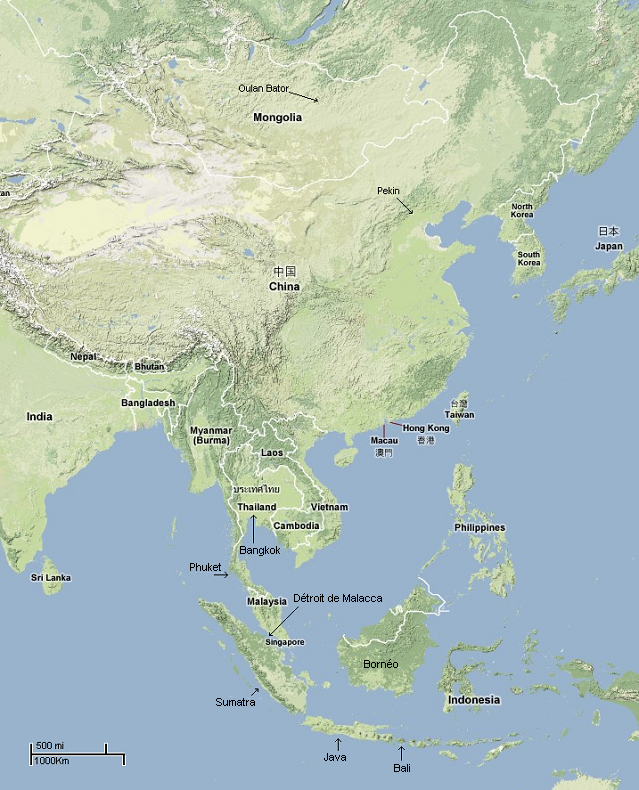
\includegraphics[width=4.8cm]{articles/C-est-bientot-reparti/trip.png}
Le trip prévu.

La suite est moins organisée, je reprends mon sac à Phuket, direction Bangkok pour aller voir une amie de mes parents qui s'appelle devinez comment... ? Cécile bien sûr... Après Bangkok direction le Laos pour aller en Chine... mais peut être, sans doute, un passage par le Vietnam (Gad je compte sur toi).

Le but final est d'aller en direction de Pekin pour prendre le train trans-mongolien jusqu'à Oulan Bator, capitale de la Mongolie.

Mais rien n'est moins sur que j'arrive jusque là, en effet je ne fais pas une course, et j'ai quelques contacts de personnes à aller voir (Cécile à Bangkok, Stéphane vers Macao), d'autre personnes avec qui je ferai sûrement une partie du trajet (Dayana, Gad, ... à confirmer).

Une contrainte : être rentré pour mi juillet car je commencerai ensuite un stage à Paris pour terminer mes études.

Voila, je pars mardi 1er avril et d'ici la je termine quelques trucs et je fais mon sac.

Au plaisir de lire vos commentaire durant ce voyage, j'essaierai de vous montrer de belles photos et faire de bons récits. A bientôt.

\end{multicols}

\bigskip
\textbf{\textsc{Commentaires}}

\medskip
Jaco a écrit le 27 mars 2008 :
\begin{displayquote}
Et bien bon vent mon ptit Dud et fait attention à la chaleur ;) Si t'en as trop ramène en un peu en Alsace !
Ciao et à la prochaine !
\end{displayquote}

\medskip
Cécile, qui fait pas le voyage a écrit le 28 mars 2008 :
\begin{displayquote}
Ah là là, plein de belles choses en perspectives, tu vas t'amuser comme un p'tit fou! Comme d'hab, ouvre grand tes mirettes, profite bien du bateau, et reviens-nous en pleine forme!
Je te fais des gros bisous.
\end{displayquote}

\medskip
Tatid a écrit le 31 mars 2008 :
\begin{displayquote}
Bon voyage Dud ! Profites en bien\dots Je suivrai tes aventures sur ton blog\dots Par contre, en tant que bon GI, tu pourrais nous faire un petit flux RSS là :-P
\end{displayquote}

\medskip
Isa a écrit le 31 mars 2008 :
\begin{displayquote}
Salut dud,
Profites en bien et n'oublie pas de nous faire partager de belles photos ça donnera envie d'y aller!
Gros bisous\dots
\end{displayquote}

\medskip
Etienne a écrit le 2 avril 2008 :
\begin{displayquote}
Ne vous inquiétez pas pour les photos, cette fois j'ai assuré le coup si j'ai des problèmes Mac se chargera de sauvegarder les photos en lieu sûr depuis une connexion internet digne de ce nom.
Ca y est c'est parti, je suis en transit à l'aéroport de Singapour, super classe !!!
A bientôt.
\end{displayquote}

\medskip
Titou a écrit le 2 avril 2008 :
\begin{displayquote}
Salut mon pti Dud ! Content de voir que la première partie de ton voyage s'est bien passée ! Profites en à fond et fais nous baver avec tes futures photos !
As we say out there, take care, enjoy and have fun !
A plus mon pote\dots
\end{displayquote}

\vfill

